\section{Trattazione teorica}

\subsection{Pianificazione locale}
\subsubsection{Superamento degli ostacoli}
Il percorso verso un obiettivo in una mappa nota viene pianificato con un algoritmo di pianificazione globale, che fornisce al robot la traiettoria dalla posa iniziale a quella desiderata. Si basa sulla conoscenza dell'intera mappa e della posizione degli ostacoli al momento della pianificazione. In fase di esecuzione, gli scenari reali possono presentare entità sconosciute o dinamiche che rappresentano le discrepanze tra modello e realtà. La maggior parte di questi problemi può essere affrontata utilizzando un pianificatore locale, un sistema che reagisce alla rilevazione di ostacoli imprevisti e riprogramma localmente la traiettoria. Le principali caratteristiche richieste per algoritmi di questo tipo sono rivolte a: 
\begin{itemize}
    \item l'obiettivo generale.
    \item la velocità e la cinematica effettive del robot.
    \item i sensori di bordo.
    \item il rischio di collisione attuale e futuro.
\end{itemize}
Si riportano di seguito, tre famiglie di approcci di pianificazione locale proposti come esempi da testi di riferimento del settore, nello specifico da "Introduction to Autonomous Mobile Robots" di R. Siegwart, I. R. Nourbakhsh e D. Scaramuzza \cite{siegwart2011introduction}.

\subsubsection{Algoritmi BUG}
BUG è una famiglia di approcci molto semplici per l'evitamento degli ostacoli, che consiste sostanzialmente nell'aggirarli per poi riprendere il percorso verso l'obiettivo. Ci concentriamo sulle tre versioni e sulle relative procedure:
\begin{itemize}
    \item BUG 0: ci si dirige verso l'obiettivo, si evitano gli ostacoli seguendone il perimetro finché non si riesce a riprendere il percorso verso l'obiettivo. Tra gli algoritmi è il più veloce e facile da implementare ma il meno affidabile, può rimanere bloccato in presenza di ostacoli complessi.
    \item BUG 1: ci si dirige verso l'obiettivo, se si incontra un ostacolo, lo si circumnaviga completamente fino a tornare al punto dove è avvenuta la collisione memorizzando per ogni punto la vicinanza alla meta e si torna al più vicino per riprendere il percorso. Garantisce di trovare il percorso ma risulta inefficiente e non ottimale.
    \item BUG 2: ci si dirige verso l'obiettivo lungo la linea $m$ (cioè la linea dall'origine alla destinazione). Se c'è un ostacolo, lo si aggira fino a quando non si incontra di nuovo la linea $m$ più vicina alla meta e dunque si lascia l'ostacolo per proseguire verso l'obiettivo. Risulta più efficiente di BUG 1 ma può non essere ottimale in scenari complessi.
\end{itemize}

\begin{figure}[h]
    \centering
    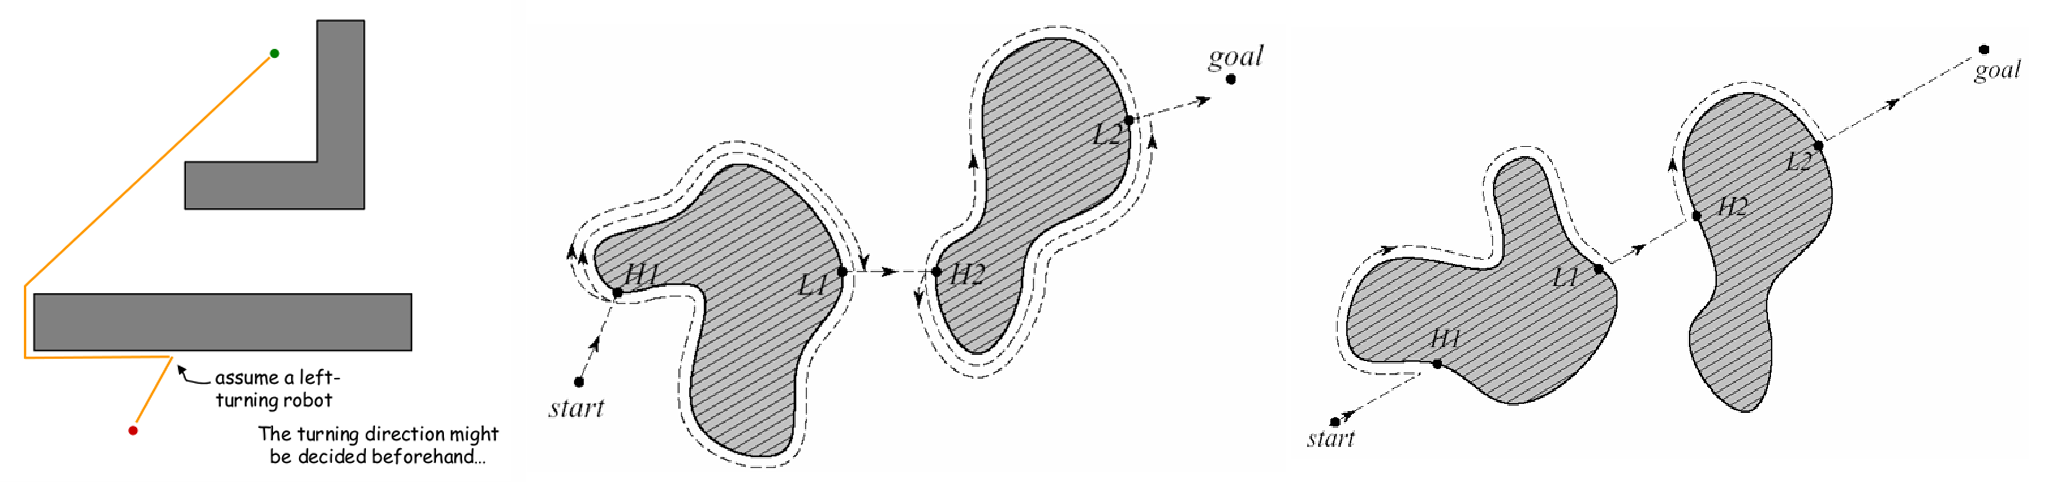
\includegraphics[width=1\linewidth]{immagini/bug_alg.png}
    \caption{BUG-0 vs BUG-1 vs BUG-2. Fonte \cite{choudhury2020design}}
    \label{fig:BUG}
\end{figure}


\subsubsection{Dynamic Window Approach}
La pianificazione locale dovrebbe tenere conto, oltre ai dati relativi ai percorsi e agli ostacoli, di altri elementi, quali, ad esempio, i vincoli sulle traiettorie e sulle velocità locali. Il Dynamic Window Approach (DWA) è un algoritmo di evitamento ostacoli in tempo reale, particolarmente usato nei sistemi di navigazione autonoma. A differenza degli algoritmi BUG, che usano strategie reattive semplici, DWA utilizza un'ottimizzazione basata su finestre di velocità per determinare la traiettoria sicura e più efficiente. La finestra dinamica limita le velocità ammissibili tenendo conto delle accelerazioni massime. La funzione obiettivo ha la forma:
\[J=\alpha \text{ heading}(v,\omega)+ \beta \text{ velocity}(v,\omega)+ \gamma \text{ distance}(v,\omega)\]
dove $heading$ denota un termine che cerca di mantenere la direzione verso l'obiettivo e il percorso globale, $velocity$ un termine che si muove il più velocemente possibile e $distance$ costringe a stare lontano dagli ostacoli. La procedura di base dell'algoritmo DWA è la seguente:
\begin{enumerate}
    \item Campionamento discreto dello spazio di controllo del robot $(v,\omega)$.
    \item Per ogni coppia di velocità campionata $(v,\omega)$, si esegue una simulazione in avanti dallo stato attuale del robot per prevedere cosa accadrebbe se la velocità campionata venisse applicata per un certo periodo di tempo (il cosiddetto orizzonte di pianificazione).
    \item Valutazione ogni traiettoria risultante dalla simulazione in avanti, utilizzando la metrica $J$, illustrata sopra, che incorpora caratteristiche quali: distanza rispetto agli ostacoli, all'obiettivo, al percorso globale e la velocità.
    \item Scarto delle traiettorie che prevedono lo scontro con gli ostacoli.
    \item Scelta la traiettoria con il punteggio di $J$ più alto e attuazione delle velocità associate da parte della base mobile.
\end{enumerate}
Dynamic Window Approach è più reattivo rispetto agli ostacoli in movimento e più fluido rispetto agli algoritmi BUG grazie all'ottimizzazione della traiettoria nel breve periodo. Questo, però, comporta un maggior costo computazionale ed il tuning dei parametri $\alpha$, $\beta$ e $\gamma$.

\subsubsection{Timed Elastic Band} 
Il Timed Elastic Band (TEB) è un algoritmo avanzato di pianificazione locale basata su grafo del movimento per robot mobili. Si basa su un modello elastico per ottimizzare la traiettoria del robot, tenendo conto di collisioni, dinamica e tempo. Le caratteristiche di base di TEB sono le seguenti:
\begin{itemize}
    \item Ottimizza localmente la traiettoria del robot e i tempi invece di selezionare le velocità migliori come DWA.
    \item La traiettoria iniziale generata da un pianificatore globale viene ottimizzata durante l'esecuzione, minimizzando il tempo richiesto per la traiettoria (obiettivo ottimale in termini di tempo), la separazione dagli ostacoli e il rispetto dei vincoli cinematici e dinamici come le velocità e delle accelerazioni massime.
    \item Il controllo predittivo basato su modello integra la pianificazione della traiettoria ottimale con il feedback di stato nel circuito di controllo
    \item L'approccio TEB formula il problema del controllo ottimo dell'orizzonte fisso per le transizioni punto-punto come un programma non lineare, scritto come un ipergrafo:
    \[f(B)=\sum_k\gamma_kf_k(B),\;\;\;B^*=arg \min_Bf(B)\]
    $f(B)$ è la funzione di costo totale che valuta ogni possibile comando di velocità $B=(v,\omega)$, Ogni $f_k(B)$ rappresenta un criterio di valutazione; ad esempio, distanza dall'obiettivo $f_{heading}$, distanza dagli ostacoli $f_{clearance}$, velocità preferita $f_{velocity}$. I pesi $\gamma_k$ bilanciano l'importanza di ogni criterio.
\end{itemize}


\subsection{Fondamenti di Reinforcement Learning}
\subsubsection{Definizione}
Il reinforcement learning (RL) è un paradigma di apprendimento automatico in cui un agente viene addestrato a eseguire azioni senza essere esplicitamente supervisionato con dati etichettati. A differenza dell'apprendimento supervisionato, in cui il segnale di supervisione è esattamente la quantità che il modello deve stimare, nel reinforcement learning si sfrutta il concetto di ricompensa, che codifica se una sequenza di scelte fatte dall'agente è vantaggiosa per la risoluzione del compito o meno. La ricompensa è l'elemento che distingue il RL da tutti gli altri paradigmi e si ottiene attraverso le interazioni tra l'agente e l'ambiente, che la fornisce in risposta alle azioni eseguite. L'agente, quindi, apprende dalle sequenze di interazioni con l'ambiente, con l'obiettivo di individuare sequenze di azioni che massimizzino la ricompensa ottenuta. 

\begin{figure}[h]
    \centering
    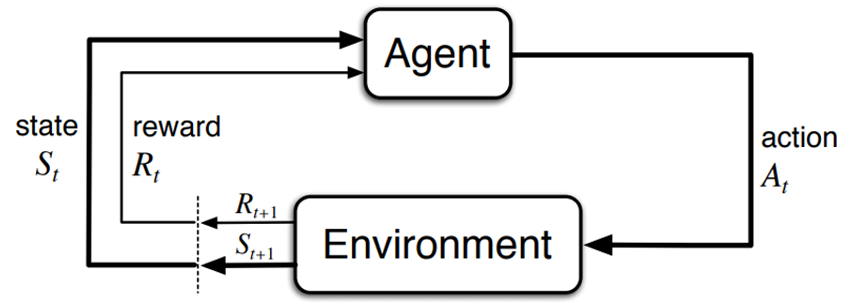
\includegraphics[width=0.4\linewidth]{immagini/reinforcement_learning_scheme.png}
    \caption{Schema esemplificativo del reinforcement learning. Fonte: \cite{sutton2018reinforcement}(figura 3.1).}
    \label{fig:rl_schema} 
\end{figure}

L'obiettivo di RL è quello di trovare una buona politica, cioè una funzione che, per ogni possibile stato, fornisca l'azione da eseguire. L'aggettivo "buona" è legato alla definizione della funzione di ricompensa, che a sua volta dipende dalle caratteristiche del compito e dai vincoli imposti. Per fornire un inquadramento formale, introduciamo alcune definizioni fondamentali per il reinforcement learning:
\begin{itemize} 
    \item Agente: entità che interagisce con l'ambiente e acquisisce le osservazioni.
    \item Ambiente: comprende tutto ciò che è al di fuori dell'agente; il suo stato potrebbe cambiare indipendentemente da quest'ultimo e dalle sue azioni.
    \item Stato: osservazione, dipendente la tempo, dell'ambiente e dell'agente. Permette a quest'ultimo di formulare una rappresentazione interna di sé e del contesto. Lo stato è un elemento del relativo spazio $\mathcal{S}$ rappresentato dal vettore $s \in R^D$ dove $D$.
    \item Azione: ciò che l'agente fa in ogni fase temporale. Così come lo stato, anche questa può essere modellata da una variabile aleatoria $a$, che codifica i possibili valori dell'azione al passo temporale $t$:
        \begin{equation}
            p(a)=Pr\{a_t=a\},\;\;\;a \in \mathcal{A}
        \end{equation}
    \item Modello: quando un'azione viene eseguita in un determinato stato, lo stato cambia (oppure no) di conseguenza. La funzione che codifica questo aspetto è la dinamica di transizione di stato. Questa funzione codifica la corrispondenza tra la coppia azione-stato e lo stato successivo che, nel caso di modello non deterministico, è una variabile aleatoria, così come la ricompensa che ne consegue. Il modello è, dunque, descritto da una distribuzione condizionale data l'azione e gli stati passati.
    \begin{equation}p(s'|s,a)=Pr\{s_{t+1}=s|s_t=s,a_t=a\}\end{equation}
    \item Politica: anche detta \textit{policy}, descrive il comportamento dell'agente, ovvero come l'agente sceglie l'azione da compiere in base allo stato in cui si trova. La politica è il risultato dell'addestramento nel reinforcement learning ed esprime l'algoritmo che dovrà compiere l'inferenza. Per brevità, da qui in avanti si prenderà in considerazione sono il caso non deterministico:
    \begin{equation}\pi(a|s)=p(a_t=a|s_t=s)\end{equation}
    \item Ricompensa: la caratteristica più distintiva del reinforcement learning. È uno scalare che definisce l'obiettivo da massimizzare (o minimizzare, nel caso della formulazione dei costi). Ogni volta che l'agente esegue un'azione in un determinato stato, l'ambiente fornisce una codifica di ricompensa che indica se l'azione è buona o meno. Quindi, la ricompensa è una funzione dello stato e dell'azione.
    \begin{equation}r(s,a)\in \mathbb{R}\end{equation}
    In generale, le ricompense elevate vengono utilizzate per incoraggiare l'agente a intraprendere le azioni corrispondenti, mentre le ricompense negative indicano che le azioni selezionate non sono utili per risolvere il compito. Tuttavia, poiché il mondo potrebbe essere stocastico, la selezione di un'azione in un certo stato potrebbe comportare diversi stati successivi e, quindi, ricompense diverse. Quindi, anche la ricompensa è modellata come una variabile aleatoria $r$. In particolare, esprimiamo la ricompensa attesa quando il sistema è allo stato $s_t = s$ e dato che l'azione $a_t = a$ è stata eseguita come il valore atteso ottenuto facendo la media delle ricompense secondo la distribuzione di transizione di stato.
    \begin{equation}r(s,a)=\mathbb{E}_{p(r|s,a)}[r_t=r|s_t=s, a_t=a]=
    \sum_{r_t \in \mathcal{R}}rp(r|s,a)=\end{equation}
    \begin{equation}=\sum_{r_t \in \mathcal{R}}r\sum_{s' \in \mathcal{S}}p(s',r|s,a), \;\;\;\forall s \in \mathcal{S},\;a \in \mathcal{A}\end{equation}
    Una policy è buona quando garantisce una ricompensa totale alta nel lungo periodo (dopo molteplici interazioni con gli ambienti). Un'azione che si traduce in un'alta ricompensa immediata, potrebbe non essere la scelta migliore a lungo termine.
    \item Fattore di sconto:  anche detto \textit{discount factor} e indicato con $\gamma \in (0,1)$, viene utilizzato per pesare le ricompense future e garantire che la serie converga a un valore finito. Se $\gamma$ è vicino a 0 si pone maggiore enfasi sui rendimenti immediati cioè la politica sarà più miope. Se $\gamma$ è vicino ad 1, invece, si prediligono i rendimenti a lungo termine, la politica sarà più lungimirante. La presenza del fattore di sconto è importante anche per unificare la formulazione per le attività episodiche e continuative.
\end{itemize}


\subsubsection{Framework Markov Decision Process}
La base teorica su cui poggia l'apprendimento per rinforzo è il Markov Decision Process (MDP) che modella il processo decisionale in situazioni in cui i risultati sono in parte casuali e in parte sotto il controllo di un decisore.
\begin{itemize}
    \item Un insieme di stati $S$ che si assume finito.
    \item Un insieme di azioni $A$, che si assume essere finito.
    \item Un modello, cioè una funzione di probabilità di transizione di stato $p(s_{t+1}|s_t,a_t)$.
    \item Funzione di ricompensa $r(s,a)$.
    \item Fattore di sconto $\gamma \in (0,1)$.
\end{itemize}
Come affermato in precedenza, l'interesse è massimizzare la ricompensa a lungo termine e non quella immediata. A questo scopo, si introduce un'ulteriore variabile casuale, ovvero il ritorno atteso $g_t$. La scelta più semplice per questo ritorno è la somma di tutte le ricompense ricevute dopo il passaggio temporale $t$:
\begin{equation}g_t=r_{t+1}+r_{t+2}+...+r_{T}\end{equation}
dove $T$ è il passo finale (una variabile aleatoria anch'essa). Una possibile classificazione dei compiti è quella che prevede: quelli che possono essere raggruppati in sotto-sequenze, detti episodici, e compiti che continuano indefinitamente, detti continui. Nel primo, $T$ è ben definito e lo stato finale in cui termina l'episodio è noto come stato terminale. Di solito, viene esteso lo spazio degli stati con questo stato terminale aggiuntivo, cioè $\mathcal{S}^+$. Le attività continue, invece, hanno $T = \infty$, quindi, la definizione di ritorno di cui sopra è problematica, poiché potrebbe divergere all'infinito (è la quantità da massimizzare); è qui che entra in gioco il fattore sconto. A condizione che $0 \leq \gamma \leq 1$ e che la ricompensa $r_t$ sia limitata, si ottiene la seguente espressione ricorsiva:
\begin{equation}g_t= r_{t+1}+\gamma r_{t+2}+\gamma^2 r_{t+3}=r_{t-1}+\gamma g_{t+1}\end{equation}


\subsubsection{Calcolo dei ritorni}
Esistono due metodi per calcolare i rendimenti: applicando direttamente la definizione, che comporta la somma di tutte le ricompense scontate lungo una traiettoria, o utilizzando il \textit{bootstrapping}. Applicando direttamente la definizione, i rendimenti si calcolano a partire da ogni stato come segue:
\begin{equation}v(s_1)=r_1+\gamma r_2+\gamma^2 r_3+...\end{equation}
\begin{equation}v(s_2)=r_2+\gamma r_3+\gamma^2 r_4+...\end{equation}
\begin{equation}v(s_3)=r_3+\gamma r_4+\gamma^2 r_5+...\end{equation}
\[...\]
Con l'idea del bootstrapping, invece, si sfruttiamo l'interdipendenza tra i rendimenti. Si calcola il rendimento di uno stato con quello di un altro (che a sua volta potrebbe dipendere dal primo). Nell'esempio, infatti, $v(s_1)$ dipende da $v(s_2)$, $v(s_2)$ dipende da $v(s_3)$, $v(s_3)$ dipende da $v(s_4)$ e $v(s_4)$ dipende a sua volta da $v(s_1)$.
\begin{equation}v(s_1)=r_1+\gamma (r_2+\gamma r_3+...)= r_1+\gamma v(s_2)\end{equation}
\begin{equation}v(s_2)=r_2+\gamma (r_3+\gamma r_4+...)= r_2+\gamma v(s_3)\end{equation}
\begin{equation}v(s_3)=r_3+\gamma (r_4+\gamma r_1+...)= r_3+\gamma v(s_4)\end{equation}
\[...\]
Il bootstrapping potrebbe sembrare meno conveniente poiché introduce un ciclo infinito di dipendenze. Tuttavia, se si scrive la relazione in forma matrice-vettore, si ottiene un risultato interessante:
\begin{equation}\begin{bmatrix}
    v(s_1)\\v(s_2)\\v(s_3)\\v(s_4)
\end{bmatrix}=\begin{bmatrix}
    r_1\\r_2\\r_3\\r_4
\end{bmatrix}+
\begin{bmatrix}
    \gamma v(s_2)\\\gamma v(s_3)\\\gamma v(s_4)\\\gamma v(s_1)
\end{bmatrix}=\begin{bmatrix}
    r_1\\r_2\\r_3\\r_4
\end{bmatrix}+\gamma
\begin{bmatrix}
    0&1&0&0\\0&0&1&0\\0&0&0&1\\1&0&0&0
\end{bmatrix}\begin{bmatrix}
    v(s_1)\\v(s_2)\\v(s_3)\\v(s_4)
\end{bmatrix}\end{equation}
che può essere scritto come:
\begin{equation}v=r+\gamma Pv\end{equation}
e il valore di $v$ può essere calcolato come $v=(I-\gamma P)^{-1}r$ (si può dimostrare che $(I-\gamma P)$ è sempre invertibile).


\subsubsection{Funzione stato-valore}
Sebbene il ritorno possa essere utilizzato per valutare le politiche, occorre tenere in considerazione la natura stocastica del framework definito. Una coppia stato-azione non restituisce sempre la stessa ricompensa, ma segue una distribuzione. Per affrontare questo problema, è necessario collegare formalmente il concetto di ritorno dallo stato. La routine di ottimizzazione viene realizzata allo scopo di trovare la politica che, a partire da ogni stato, fornisca il massimo rendimento possibile. In particolare, è necessario introdurre il concetto di Value Function, una funzione dello stato che esprime il rendimento atteso che osserviamo a partire da esso. Si consideri una sequenza di passi temporali $t=0,1,2,...$, al momento $t$ l'agente è nello stato $s_t$ e l'azione intrapresa a seguito di una politica $\pi$ è $a_t$. Lo stato successivo è $s_{t+1}$ e la ricompensa immediata ottenuta è $r_{t+1}$:
\begin{equation}s_t\xrightarrow[]{a_t} s_{t+1},r_{t+1}\end{equation}
Tutti i termini, cioè $s_t$, $s_{t+1}$, $a_t$, $r_{t+1}$ sono variabili aleatorie. A partire da $t$, si ottiene una sequenza stato-azione-ricompensa:
\begin{equation}s_t\xrightarrow[]{a_t} s_{t+1},r_{t+1} \xrightarrow[]{a_{t+1}} s_{t+2},r_{t+2}\xrightarrow[]{a_{t+2}} s_{t+3},r_{t+3}...\end{equation}
Richiamando la definizione si scrive il ritorno atteso come:
\begin{equation}g_t=r_{t+1}+\gamma r_{t+2}+\gamma^2 r_{t+3}+...\end{equation}
dove $\gamma \in (0,1)$ è il fattore di sconto. Si noti che anche $g_t$ è una variabile aleatoria poiché lo sono le ricompense. Quindi, è possibile calcolare il suo valore atteso:
\begin{equation}v_\pi (s)= \mathbb{E}[g_t=g|s_t=s]\end{equation}
chiamata funzione stato-valore (state-value function). Dipende da $s$ poiché l'aspettativa dei rendimenti è calcolata a partire da $s$, e da $\pi$ poiché le traiettorie sono generate secondo una politica. La state-value è calcolata considerando l'intera traiettoria e non una specifica fase temporale o parte di essa. La formulazione della funzione stato-valore più utilizzata è l'equazione di Bellman che, nel caso della politica $\pi$ può essere scritta come:
\begin{equation}v_\pi (s)= \mathbb{E}[g_t=g|s_t=s]=\sum_{a \in \mathcal{A}}\pi(a|s)\sum_{s'\in \mathcal{S}}\sum_r p(s',r|s,a)[r+\gamma v_\pi(s')]\end{equation}


\subsubsection{Funzione azione-valore}
Mentre la funzione stato-valore descrive il rendimento atteso ottenibile a partire da uno stato, la funzione action-value esprime il rendimento atteso ottenibile partendo da uno stato e intraprendendo una certa azione. Questa funzione è definita come:
\begin{equation}q_\pi(s,a)=\mathbb{E}[g_t=g|s_t=s,a_t=a]\end{equation}
Pertanto, si ricava:
\begin{equation}v_\pi(s)=\sum_{a \in \mathcal{A}}\pi(a|s)q_\pi(s,a)\end{equation}
Si potrebbe pensare che per le azioni mai selezionate da una politica il $q_\pi(s,a)$ sia zero. Tuttavia, non è così; sebbene l'azione non sia selezionata dal criterio, ha comunque un valore che può essere calcolato osservando cosa accadrebbe quando selezionata in quello stato. In secondo luogo, tale azione potrebbe non essere selezionata dall'attuale politica, il che potrebbe non essere ottimale. Al fine di trovare una politica migliore, è importante esplorare anche i valori delle azioni che non sono selezionate dalla politica attuale. Per ottenere l'equazione di Bellman per la funzione azione-valore, si può rimuovere semplicemente la media delle azioni per lo stato corrente dall'equazione di Bellman della funzione del valore dello stato:
\begin{equation}q_\pi(s,a)= \sum_{r\in R} p(r|s,a)r+\gamma \sum_{s'\in \mathcal{S}}p(s'|s,a)\sum_{a' \in \mathcal{A}(s')}\pi(a'|s')q_\pi(s',a')\end{equation}


\subsubsection{Politiche ottimali}
Una politica $\pi^*$ è ottimale se $v_\pi^*(s) \geq v_\pi(s)$, $\forall s \in \mathcal{S}$ e per qualsiasi altra policy $\pi$. Ciò non garantisce garanzie riguardo all'esistenza, l'unicità di tale politica né fornisce l'algoritmo per calcolarla. A questo scopo si introduce l'equazione di ottimalità di Bellman (BOE) che codifica la massimizzazione della funzione stato-valore rispetto alla policy:
\begin{equation}v(s)= \max_{\pi(s)\in \Pi(s)}\sum \pi(a|s)q(s,a)\end{equation} 
Dati i teoremi che affermano l'esistenza e l'unicità della soluzione, si ricava la politica ottimale $\pi^*$ attraverso una strategia greedy\footnote{algoritmo che effettua ad ogni passo la scelta localmente ottima} come suggerito dal teorema: per ogni $s \in \mathcal{S}$, la politica deterministica
\begin{equation}\pi^*(a|s)=\begin{cases}
    1\;\;\;\text{ se $a=a^*(s)$}\\
    0\;\;\;\text{ se $a\neq a^*(s)$}
\end{cases}\end{equation}
è una politica ottimale per la BOE. Si noti, inoltre, che:
\begin{equation}a^*(s)=arg \max_a q^*(a,s)\end{equation}
dove
\begin{equation}q^*(s,a)=\sum_{r\in R}p(r|s,a)+\gamma \sum_{s'\in S}p(s'|s,a)v^*(s')\end{equation}


\subsection{Approcci RL}
\subsubsection{Classificazione}
Definiti i principi fondamentali dell'apprendimento per rinforzo, si fornisce una panoramica dei possibili approcci e delle rispettive peculiarità. La principale distinzione è quella tra gli approcci tabulari e quelli non tabulari; i primi sfruttano una rappresentazione matriciale per codificare la corrispondenza tra state-value function e gli elementi nello spazio di stato. Questo metodo è vantaggioso in termini di calcolo, ma diventa oneroso dal punto di vista della memoria se lo scenario impone spazi di stato grandi e complessi. Gli approcci non tabulari rinunciano a conservare il valore esatto della funzione per ogni singolo stato da aggiornare ad ogni iterazione. Questo conferisce diversi vantaggi: li rende adatti a spazi di stato molto grandi o continui, garantisce una maggiore efficienza in termini di memoria e fornisce una migliore capacità di generalizzazione. Vista la natura della trattazione presente si è scelto di prendere in considerazione solo quest'ultimi. 

% approcci non tabulari
Gli approcci non tabulari, anche detti \textit{Approximate Solution Methods}, si dividono in diverse famiglie. Le più rilevanti per il caso in esame sono: 
\begin{itemize}
    \item Value-based: prevedono di approssimare la state-value function, derivando la politica dalla scelta greedy o $\epsilon$-greedy dell'azione. Fanno parte di questi metodi: Deep Q-learning, Montecarlo VFA e SARSA VFA.
    \item Policy Gradient: apprendono direttamente una politica parametrica $\pi_\theta(a|s)$, senza stimare la state-value function ma con l'utilizzo di gradienti per la stima dei parametri ottimi. Gli approcci più comuni sono: Reinforce, Deterministic Policy Gradient (DPG) e Proximal Policy Optimization (PPO).
\end{itemize}
% confronto
I metodi Value-based sono i più semplici da implementare, ma soffrono particolarmente nelle applicazioni con spazio degli stati continuo e ad alta dimensionalità. Per questo motivo l'utilizzo nel controllo robotico è molto limitato rispetto agli altri approcci. I metodi Policy Gradient, invece, sono adatti ad ambienti ad elevata dimensionalità e apprendono politiche stocastiche ottimali. L'elevata varianza nei gradienti, però, può rendere l'apprendimento instabile. Questi approcci sono ampiamente utilizzati nella robotica AI-based. 


\subsubsection{Metodi Policy Gradient}
Secondo Sutton e Barto \cite{sutton2018reinforcement}, i metodi Policy Gradient sono una categoria di approcci nell'apprendimento per rinforzo che non stimano esplicitamente la state-value function ma ottimizzano direttamente la policy in modo da massimizzare le ricompense. La politica $\pi_\theta(a|s,\theta)$ viene, dunque, parametrizzata arbitrariamente attraverso dei $\theta$ che devono essere addestrati; l'unica condizione è la conservazione della differenziabilità. Ad esempio, se lo spazio delle azioni è discreto, è possibile utilizzare una rete neurale per stimare una funzione che preveda le ricompense per ogni azione e quindi utilizzare una funzione \textit{softmax} per ottenere la seguente policy parametrizzata:
\begin{equation}\pi(a|s,\theta)=\frac{e^{h(a,s,\theta)}}{\sum_{a \in \mathcal{A}}e^{h(b,s,\theta)}}\end{equation}
Occorre definire una funzione obiettivo $J(\theta)$ che esprima la bontà della parametrizzazione al tempo $t$ e permetta di calcolare il nuovo $\theta$ per migliorare tale obiettivo. Si scrive, dunque, un semplice ottimizzatore:
\begin{equation}\theta_{t+1}\xleftarrow{}\theta_t +\alpha \nabla_\theta \hat{J}(\theta_t)\end{equation}
dove $\alpha$ è il tasso di apprendimento e $\nabla_\theta \hat{J}(\theta_t)$ è la stima del gradiente della funzione obiettivo.

% Reinforce
Ronald J. Williams, in un suo articolo \cite{williams1992simple} del 1992, propone il primo algoritmo di questa famiglia, Reinforce. Questo approccio introduce la seguente funzione obiettivo:
\begin{equation}
    J(\theta)= \mathbb{E}_{\tau\sim \pi_\theta}[R(\tau)]
\end{equation}
dove $\tau= (s_0,a_0,r_0,s_1,a_0,r_1,...)$ è la traiettoria generata dalla politica $\pi$ ed $R(\tau)$ è la somma delle ricompense scontate. A partire dalla funzione obiettivo si calcola il gradiente come segue:
\begin{equation}
    \nabla_\theta \hat{J}(\pi_\theta) = \int_\mathcal{S} \rho^\pi \int_\mathcal{A} \nabla_\theta \pi_\theta(a|s) q^\pi(s,a) da ds
    =\mathbb{E}_{s\sim\rho^\pi,a\sim\pi_\theta}{\nabla_\theta \log (\pi_\theta(a|s)q^\pi(s,a))}
\end{equation}
dove $\rho^\pi(s)$ è la probabilità dello stato. Richiamando l'algoritmo di ascesa del gradiente si scrive l'ottimizzatore per massimizzare $J(\theta)$:
\begin{equation}\theta_{t+1}\xleftarrow{} \theta_t+\alpha\mathbb{E}[\ln(\pi(A|S;\theta_t)\cdot q_\pi(S,A))]\end{equation}
dove $\alpha > 0$ è un tasso di apprendimento costante. Poiché il vero gradiente è sconosciuto, lo sostituiamo con uno stocastico:
\begin{equation}\theta_{t+1} \xleftarrow{}\theta_t+\alpha \nabla_\theta \cdot \ln(\pi(a_t|s_t;\theta_t)\cdot q_t(s_t,a_t))\end{equation}
dove $q_t(s_t,a_t)$ è un'approssimazione di $q_\pi(s_t,a_t)$. L'idea centrale è quella di massimizzare la \textit{score function}\footnote{misura la bontà in termini di ricompense} $\nabla_\theta log(\pi_\theta(a|s))$ della politica. Le criticità di questo approccio sono: l'alta varianza nella stima del gradiente e l'inefficienza campionaria dovuta al fatto che l'ottimizzazione avvenga solo a valle di un episodio.


\subsubsection{Sottofamiglia Actor-Critic}
Gli approcci Actor-Critic combinano le strategie Value-based con quelle Policy Gradient, infatti, alcuni testi \cite{sutton2018reinforcement}, li considerano una sottofamiglia di quest'ultimi. Storicamente risultano precedenti a Reinforce essendo stati introdotti da Sutton in una sua pubblicazione \cite{sutton1984temporal} del 1984, ma rappresentano la soluzione migliore alle sue criticità. L'idea principale è quella di separare il processo decisionale, cioè quello che implementa la politica, da quello valutativo, ossia quello che esamina le ricompense. Il primo compito viene svolto dall'entità \textit{actor} che ricava le azioni dalla politica parametrica mentre il secondo dalla \textit{critic} che approssima la state-value function e guida l'apprendimento attraverso un feedback. L'actor aggiorna la policy tramite ascesa del gradiente:
\begin{equation}
     \nabla_\theta J(\theta)\approx\nabla_\theta \log\pi_\theta(a_t|s_t)\cdot \hat{A}(s_t,a_t)
\end{equation}
dove $\hat{A}(s_t,a_t)$ è una stima del vantaggio ossia quanto l'azione abbia portato ricompense migliori del valore atteso. Il critic stima la state-value function attraverso un approccio Temporal Difference\footnote{famiglia di algoritmi di RL che stima i ritorni durante l'episodio tramite bootstrapping, senza attendere la sua terminazione}:
\begin{equation}
    v_{t+1}(s_t)=v_t-\alpha_v\delta_t=v_t-\alpha_v[r_{t+1}+\gamma v_\pi(s_{t+1})-v_t(s_t)]
\end{equation}
Formalmente il vantaggio $A(s_t,a_t)$ consiste nella differenza tra action-value function e state-value function calcolate nell'istante $t$ per l'azione selezionata ma spesso viene usata una versione approssimata che riduce la varianza:
\begin{equation}
    A(s_t,a_t)=q(s_t,a_t)-v(s_t)\approx \delta_t=r_t+\gamma v(s_{t+1})-v(s_t)
\end{equation}
Calcolati il gradiente della funzione obiettivo e la state-value function, l'actor usa il primo per calcolare i parametri della policy:
\begin{equation}
    \theta_{t+1}\xleftarrow{} \theta_t+\alpha \nabla_\theta J(\theta)
\end{equation}
ad il critic usa la seconda per ridurre l'errore di Temporal Difference:
\begin{equation}
    w\xleftarrow{} w+\alpha_v \nabla_w [\delta_t^2]
\end{equation}
La famiglia Actor-Critic garantisce maggiore stabilità ed efficienza rispetto ai metodi basati solo sulla stima della politica come Reinforce. Come sottolineato dallo stato dell'arte, queste caratteristiche la rendono la più adatta all'ambito robotico, motivo per cui si è scelto di focalizzarsi su di essa. Da questa prima formulazione la famiglia di approcci Actor-Critic si è allargata moltissimo; di seguito si riportano tre tra gli approcci più in voga nell'ambito dell'apprendimento robotico:

\begin{itemize}
    \item Deep Deterministic Policy Gradient (DDPG): Lillicrap et al. lo formalizzano nel 2015 \cite{lillicrap2015continuous}, si tratta di un algoritmo che addestra una politica deterministica ed impone spazi di stato e di azioni continui. La caratteristica che lo distingue dagli altri approcci è la scelta di far apprendere al critic la action-value function. Per mitigarne la possibile sovrastima\footnote{l'action value richiede il calcolo del massimo che su un insieme di stime rumorose tende a essere sovrastimato in media} si introduce una seconda entità critic in modo da poter scegliere tra due alternative il valore minore. Questa variante è detta Twin Delayed Deep Deterministic Policy Gradient (TD3) e, come discusso nell'articolo \cite{li2024path}, apporta diverse migliorie rispetto a DDPG.
    \item Proximal Policy Optimization (PPO): proposto nel 2017 da Schulman e colleghi \cite{schulman2017proximal}, introduce una funzione obiettivo che limita la variazione della politica tra aggiornamenti successivi. Questo è ottenuto attraverso una funzione di \textit{clipping} che impedisce aggiornamenti troppo grandi, migliorando la stabilità dell'apprendimento. Per questo risulta ampiamente più utilizzato di metodi precedenti come Reinforce. Ad esempio nel progetto dell'Istituto Bernoulli di Groeningen \cite{wang2022ippo} viene utilizzato per l'evitamento ostacoli di un manipolatore a 6 gradi di libertà. Ne esistono versioni migliorate adattate al compito del controllo robotico.
    \item Soft Actor-Critic (SAC): introdotto da Tuomas Haarnoja e colleghi in un articolo del 2018 \cite{haarnoja2018soft}, estende l'obiettivo tradizionale dell'apprendimento per rinforzo includendo un termine di entropia, incentivando l'agente a esplorare azioni più diversificate. Questo approccio aiuta a prevenire la convergenza prematura su politiche subottimali e migliora la robustezza dell'apprendimento. SAC, rispetto ai suoi predecessori, migliora l'efficienza campionaria e si adatta ad ambienti continui e dinamici come evidenziato dall'articolo dell'IEEE \cite{nakhleh2023sacplanner} che ha messo alla prova SAC in uno scenario reale ottenendo ottimi risultati in termini di reattività con soli diecimila episodi di addestramento.
\end{itemize} 

Esistono diversi studi che propongono confronti tra questi ed altri algoritmi per valutarne l'applicazione nel controllo robotico continuo. Si è scelto di fare riferimento all'articolo del 2025 di Meta \cite{wan2025empirical} che confronta i rendimenti di PPO, TD3, SAC e DDPG introducendo dei reset che permettono di uscire da minimi locali e ottimizzare l'apprendimento. In particolare, lo studio propone tre scenari: uno senza reset, uno con reset predeterminati ed uno con reset controllati dagli agenti. SAC ha ottenuto i migliori rendimenti complessivi, specialmente in compiti complessi come \textit{HumanoidStandup}, dove ha superato significativamente gli altri algoritmi. TD3 ha fornito buoni risultati in alcuni scenari; PPO restituisce prestazioni insufficienti in scenari senza reset. Il peggiore risulta DDPG, che dimostra instabilità e fallisce in diverse occasioni. L'articolo, inoltre, segnala il miglioramento delle prestazioni di tutti gli algoritmi presi in esame in corrispondenza di reset predefiniti. Risulta, invece, persino dannoso fornirne il controllo agli agenti.

% ancora?

\subsubsection{Soft Actor-Critic}
Soft Actor-Critic è un algoritmo di Deep Reinforcement Learning quindi sfrutta le reti neurali per l'addestramento dell'agente, nel caso specifico se ne adottano tre: una guida l'actor elaborando una politica stocastica, producendo una distribuzione di probabilità sulle azioni date le osservazioni e gli altri due rappresentano dei critic che apprendono due action-value function. Questa architettura è proposta in evoluzioni recenti di SAC e affronta il problema della sovrastima dei valori di action-value, scegliendo tra le stime delle due reti il valore minimo. A differenza di algoritmi come DDPG o TD3 che utilizzano politiche deterministiche, SAC impiega una politica stocastica, permettendo all'agente di apprendere distribuzioni di azioni multimodali e migliorando l'esplorazione in ambienti con molteplici soluzioni ottimali locali. 

Di seguito si riporta la descrizione del supporto teorico di Soft Actor-Critic presente nella documentazione di OpenAI \cite{openaiSAC2023}. L'obiettivo di SAC è massimizzare la somma dei ritorni attesi e dell'entropia della politica:
\begin{equation}
    \pi^*= \arg \max_\pi \mathbb{E}_{(s_t,a_t)\sim \rho_\pi}[\sum_{t=0}^\infty\gamma^t (r(s_t,a_t)+ \alpha \mathcal{H}(\pi(\cdot|s_t)))]
\end{equation}
dove $\alpha$ è un iperparametro che bilancia l'impatto dell'entropia e $\mathcal{H}(\pi(\cdot|s_t))$ è l'entropia della politica nello stato $s_t$. Presa in esame una distribuzione di probabilità $p$:
\begin{equation}
    H(p)= \mathbb{E}_{z\sim p}[-\log p(x)]
\end{equation}
una metrica che misura la "quantità di informazione" o l'"imprevedibilità" della variabile aleatoria $x$. Questo termine è utilizzato per spronare l'agente ad esplorare; questo migliora molto le prestazioni in ambienti complessi e dinamici in cui politiche di solo sfruttamento\footnote{propensione alla scelta di soluzioni greedy, localmente ottime} possono portare a cadere in minimi locali. La state-value function va adattata alla presenza del termine entropico:
\begin{equation}
    v_\pi(s)= \mathbb{E}_{(s_t,a_t)\sim \rho_\pi}[\sum_{t=0}^\infty \gamma^t(r(s_t,a_t)+ \alpha \mathcal{H}(\pi(\cdot|s_t)))|s_0=s]
\end{equation}
così come la action-value function:
\begin{equation}
    q_\pi(s)= \mathbb{E}_{(s_t,a_t)\sim \rho_\pi}[\sum_{t=0}^\infty \gamma^t(r(s_t,a_t)+ \alpha \mathcal{H}(\pi(\cdot|s_t)))|s_0=s,a_0=a]
\end{equation}
Da cui si può ricavare la Bellman equation come segue:
\begin{equation}
    q_\pi(s,a) =  \mathbb{E}_{(s_t,a_t)\sim \rho_\pi}[R(s,a)+\gamma(q_\pi(s',a')+\alpha \mathcal{H}(\pi(\cdot|s'))]= \mathbb{E}_{(s_t,a_t)\sim \rho_\pi}[R(s,a)+\gamma v_\pi(s')]
    \label{eq:BellmanAC}
\end{equation}
Utilizzando la definizione di entropia adattiamo l'equazione \ref{eq:BellmanAC} di conseguenza:
\begin{equation}
    q_\pi(s,a) =  \mathbb{E}_{(s_t,a_t)\sim \rho_\pi}[r(s,a)+\gamma(q_\pi(s',a')-\alpha \log\pi(a'|s')]
    \label{eq:BellmanAC_alt}
\end{equation}
Non avendo a disposizione i valori futuri, occorre riscrivere la relazione \ref{eq:BellmanAC_alt} con dei termini approssimati che la rendano realizzabile:
\begin{equation}
    q_\pi(s,a) \approx \gamma (q_\pi(s',\Tilde{a}')-\alpha \log\pi(\Tilde{a}'|s'))\;\;\;\;\text{ dove }\;\Tilde{a}'\sim \pi(\cdot|s')
\end{equation}
I due critic forniscono due stime diverse dell'action-value calcolato come descritto e si decide di tenere in considerazione il valore minore. Ottenuto $q_\pi(s,a)$, è possibile calcolare la loss function utilizzando una metrica Mean Square Bellman Error (MSBE):
\begin{equation}
    L(\phi,\mathcal{D})= \mathbb{E}_{(s,a,r,s')\sim\mathcal{D}}[(q_\phi(s,a)-y(r,s',d))^2]
\end{equation}
dove $y(r,s',d)$ è la funzione di target, composta come segue:
\begin{equation}
    y(r,s',d)=r + \gamma(1-d) (\min_{j=1,2}q_\phi(s',\Tilde{a}')-\alpha \log\pi_\theta(\Tilde{a}'|s'))\;\;\;\; \text{ dove }\;\Tilde{a}'\sim \pi_\theta(\cdot|s')
\end{equation}
L'obiettivo dell'ottimizzazione è massimizzare i ritorni attesi futuri e l'entropia attesa futura. La documentazione Spinning Up di OpenAI \cite{openaiSAC2023} suggerisce il cosiddetto \textit{reparametration trick} in cui la distribuzione relativa alla politica $\pi_\theta(\cdot|s')$ viene campionata attraverso un calcolo deterministico che coinvolge lo stato, i parametri della politica e del rumore indipendente:
\begin{equation}
    \Tilde{a}_\theta (s,\xi) = \tanh (\mu_\theta(s)+\sigma_\theta(s)\odot\xi) \;\;\;\; \text{ dove }\;\ \xi \sim \mathcal{N}(0,I)
\end{equation}
A seguire la riformulazione della state-value function:
\begin{equation}
     v_\pi(s)= \mathbb{E}_{(s_t,a_t)\sim \rho_\pi}[q_\pi(s,a)-\alpha \log\pi(a|s)]=\mathbb{E}_{(\xi\sim \mathcal{N}}[q_\pi(s,\Tilde{a}_\theta(s,\xi))-\alpha \log \pi_\theta(s,\Tilde{a}_\theta(s,\xi))|s]
\end{equation}
Il passo finale è la sostituzione nella loss function di $q_\pi$ con la minore tra quelle approssimate dalle due reti $\min_{j=1,2} q_\phi^j$. Di conseguenza scriviamo
\begin{equation}
    \max_\theta \mathbb{E}_{s\sim\mathcal{D},\xi\sim \mathcal{N}}[\min_{j=1,2} q_\phi^j(s,\Tilde{a}_\theta(s,\xi))-\alpha \log \pi_\theta(\Tilde{a}_\theta(s,\xi)|s)]
\end{equation}

\begin{figure}[h!]
    \centering
    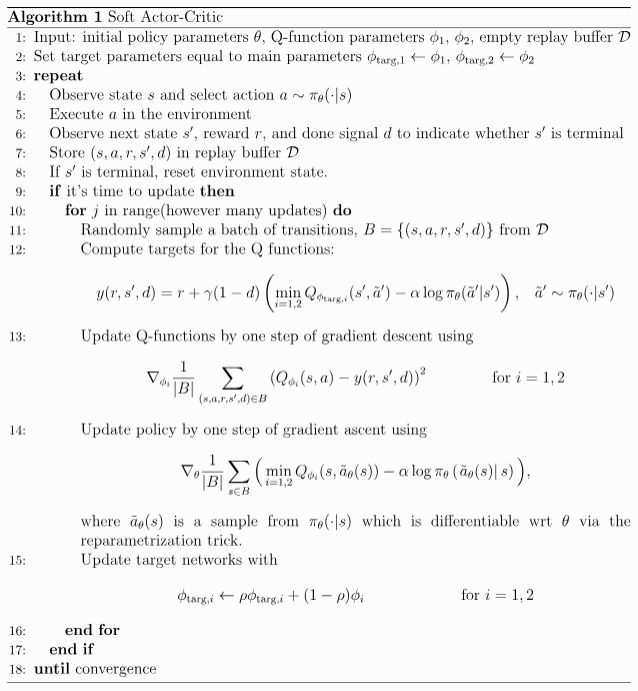
\includegraphics[width=0.65\linewidth]{immagini/sac_algo.png}
    \caption{Pseudocodice di Soft Actor-Critic. Fonte: \cite{openaiSAC2023}}
    \label{fig:sac_algo}
\end{figure}

In figura \ref{fig:sac_algo} una possibile descrizione in pseudocodice dell'algoritmo di Soft Actor-Critic.


\subsection{Reti neurali profonde}
\subsubsection{Deep Reinforcement Learning}
Come descritto in precedenza, Soft Actor-Critic appartiene agli algoritmi di reinforcement learning che adottano reti neurali profonde. Questo permette di sfruttare la capacità di stima non lineare del deep learning per approssimare le funzioni tipiche dell'ambito reinforcement come action-value function e state-value function. SAC si distingue dagli altri approcci RL per l'utilizzo di una politica stocastica, ulteriore stima che è possibile affidare alle reti profonde. In altre parole, la natura continua e non lineare delle funzioni caratteristiche dell'actor (politica) e del critic (action-value) richiede stimatori potenti e orientati alla generalizzazione, caratteristiche che contraddistinguono le reti neurali profonde. Rispetto allo scenario in esame, queste rappresentano la soluzione migliore per tradurre input grezzi, come le osservazioni del robot, in azioni senza bisogno di \textit{feature estractor}\footnote{algoritmi che ricavano feature da input ad alta dimensionalità come immagini o point cloud LiDAR} o altri moduli di preprocessing. L'intuizione di combinare reti profonde e reinforcement learning è riconducibile allo studio di DeepMind del 2013 \cite{mnih2013playing} che introduce una variante dell'algoritmo Q-learning, battezzata per l'occasione Deep Q-learning (DQN), in cui la state-value function viene stimata da una rete profonda. DQN viene messo alla prova con sette videogiochi per Atari 2600, alla rete vengono forniti i pixel dello schermo e viene richiesto di compiere un'azione nel gioco. I risultati riportati mostrano la superiorità quasi totale\footnote{dimostra prestazioni migliori in sei videogiochi su sette} del nuovo algoritmo rispetto allo stato dell'arte e, in tre occasioni, anche nei confronti del giocatore umano. 

\subsubsection{Reti neurali}
L'introduzione alle reti neurali non può che passare dal parallelismo con la struttura del cervello umano e la conseguente modellazione matematica del neurone e del legame sinaptico (vedi Figura \ref{fig:neuron}). Il neurone è l’unità computazionale di base del cervello umano, che ne contiene circa 86 miliardi, interconnessi da $10^{14}$–$10^{15}$ sinapsi. Ogni neurone riceve input tramite i \textit{dendriti} e trasmette output attraverso un singolo \textit{assone}, che si collega ai dendriti di altri neuroni. Per quanto riguarda il modello computazionale, gli input $x_i$ vengono ponderati dai pesi sinaptici $w_i$, che determinano l’intensità e la natura dell’interazione: eccitatoria (peso positivo) o inibitoria (peso negativo). I segnali ponderati vengono sommati; se la somma supera una soglia, il neurone si attiva. Questo fenomeno è modellato tramite una funzione di attivazione $f$, che restituisce il livello di risposta del neurone in uscita. 

\begin{figure}[h]
    \centering
    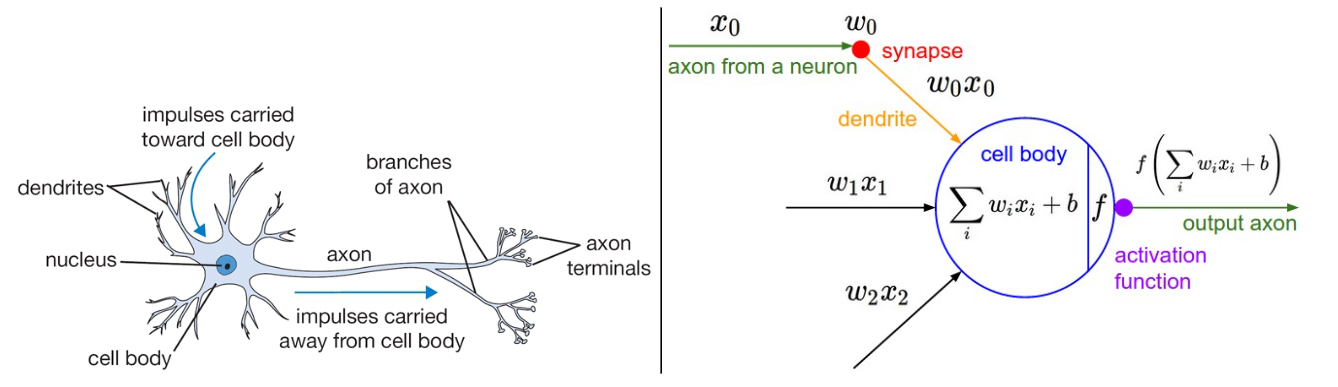
\includegraphics[width=0.85\linewidth]{immagini/neurone_umano_virtuale.png}
    \caption{Neurone umano a sinistra e modello matematico a destra. Fonte \cite{smart2023balappan}}
    \label{fig:neuron}
\end{figure}

Nella realizzazione di una rete neurale, la scelta della corretta funzione di attivazione è cruciale e deve rispettare due vincoli: derivabilità e non linearità. Ne esistono diverse con rispettivi vantaggi e svantaggi, la più diffusa è Rectified Linear Unit ($ReLU$) con le sue varianti. Nella sua forma di base si scrive:

\begin{equation}
    ReLU(x)= max\{0,x\}
\end{equation}

La \textit{backpropagation}\footnote{abbreviazione di backward propagation of errors} è l'algoritmo fondamentale per l’addestramento delle reti neurali. Esso consente di minimizzare una funzione di perdita $\mathcal{L}$ aggiornando i pesi attraverso il calcolo efficiente del gradiente dell’errore, applicando il teorema della derivata composta. Il processo si articola in tre fasi:

\begin{enumerate}
    \item Forward pass: l’input attraversa la rete producendo un’uscita.
    \item Calcolo dell’errore: in caso di apprendimento supervisionato si misura la differenza tra uscita predetta e il valore da stimare mediante una funzione di perdita.
    \item Backward pass: l’errore viene propagato all’indietro calcolando i gradienti rispetto ai pesi di ogni "sinapsi" della rete.
\end{enumerate}

L’aggiornamento dei pesi avviene secondo relazioni simili alla seguente:

\begin{equation}
    w_{ij}^{(t+1)} = w_{ij}^{(t)} - \eta \frac{\partial \mathcal{L}}{\partial w_{ij}}
\end{equation}

dove \(w_{ij}\) è il peso tra i neuroni \(i\) e \(j\) e \(\eta\) è il tasso di apprendimento. Le reti neurali sono strutture organizzate in grafi aciclici diretti, in cui gli output dei neuroni allo strato $i$ fungono da input per quelli allo strato $i+1$. L'assenza di cicli garantisce la corretta propagazione dell’informazione in avanti, mentre la disposizione in strati permette una migliore organizzazione ed una scalabilità più semplice. In particolare, i neuroni che ricevono i dati in ingresso alla rete appartengono all'\textit{input layer}, quelli che forniscono l'uscita finale della rete, invece, all'\textit{output layer} mentre tutti gli altri che risiedono negli strati intermedi fanno parte degli \textit{hidden layer}. 

Non si approfondirà ulteriormente, ma esistono molti aspetti di fondamentale importanza che occorre affrontare nella progettazione delle reti neurali come: il dimensionamento della rete, il trattamento dei dati in ingresso, l'inizializzazione dei pesi, la regolarizzazione a valle del layer, la scelta della funzione di perdita, l'ottimizzatore e altri iperparametri.


\subsubsection{Evoluzione in profondità}
Dal punto di vista teorico, le reti neurali godono del teorema che, all'apparenza, suggerisce una sorta di onnipotenza nella stima di funzioni non lineari.

\begin{theorem}[Teorema di approssimazione universale]
    Una rete feedforward con un output layer lineare e almeno un hidden layer con una funzione di attivazione non lineare (come ReLU) può approssimare "qualsiasi" funzione con errore diverso da zero, a condizione che la rete disponga di un numero sufficiente di neuroni.
\end{theorem}

Il teorema afferma l'esistenza di un numero di neuroni dell'hidden layer grazie a cui la rete riesce ad approssimare una funzione complessa, ma non garantisce che questo avvenga in tempo finito né fornisce un modo per calcolare quanti neuroni sono necessari. Se la funzione che vogliamo approssimare è complessa, potrebbe richiedere un numero esponenziale di neuroni rispetto al suo grado. Un singolo strato con così tanti neuroni non indica alcuna prior\footnote{conoscenza a priori} sul modello, il ché può rendere il processo di apprendimento ancora più difficile. La soluzione è dare profondità alla rete, più hidden layer e meno neuroni per strato. Questo significa dire alla rete di approssimare funzioni più semplici in ogni strato per poi combinarle così da distribuire la complessità, apprendendo più funzioni semplici per poi combinarle. Una rete profonda è più facile da addestrare rispetto a un singolo strato con un numero elevato di neuroni.

\begin{figure}[h]
    \centering
    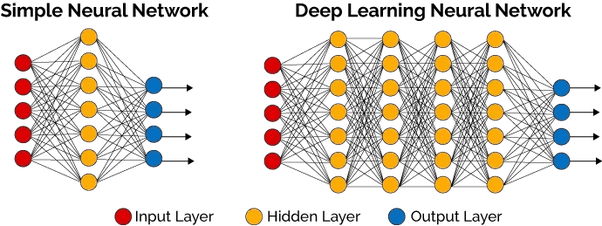
\includegraphics[width=0.6\linewidth]{immagini/deep_neural_network.png}
    \caption{Profondità delle reti neurali. Fonte: \cite{rosi2025vea}}
    \label{fig:deep_neural}
\end{figure}

Formalmente, una rete si dice profonda se ha più di un hidden layer; ma, allo stato dell'arte attuale, sono state addestrate reti con decine o centinaia di strati. Nulla vieta di costruirne anche da migliaia di layer, ma l'efficienza e la stabilità tendono a calare drasticamente. Per semplicità, è stata descritta l'architettura più classica per le reti profonde, MultiLayer Perceptron (MLP), che prevede una connessione densa in cui ogni neurone del livello $i$-esimo contribuisce all'ingresso di ogni neurone al livello  $i+1$-esimo. In realtà, col tempo, le strutture si sono diversificate, confluendo in tre grandi famiglie:
\begin{itemize}
    \item MultiLayer Perceptron (MLP): descritta in precedenza, usata principalmente per previsioni e stime su dati numerici.
    \item Convolutional Neural Network (CNN): strutture pensate per l'elaborazione di immagini, sfruttano il principio di località, cioè al tendenza dei gruppi di pixel vicini ad avere una relazione semantica, e quindi è utile processarli congiuntamente. Utilizzano filtri (\textit{kernel}) che scorrono sull'immagine (operazione di convoluzione) per estrarre feature locali con grado di astrazione crescente, come bordi, angoli, texture.
    \item Recurrent Neural Network (RNN): pensate per input sequenziali come video, audio e serie temporali, mantengono uno stato interno (\textit{hidden state}) che viene aggiornato a ogni passo temporale, permettendo alla rete di memorizzare informazioni sui dati precedenti. Questo permette di valutare in ogni istante il contributo delle elaborazioni precedenti su quella attuale.
\end{itemize}

Occorre ricordare, inoltre, che esistono innumerevoli combinazioni di strutture multi-rete che rispondono ad esigenze diverse tra loro come GAN, Trasformer ed Encoder-Decoder. 


\subsection{Sensor fusion}

\subsection{Simulazione}